\documentclass[final]{beamer}

\usepackage[scale=1.24]{beamerposter} % Use the beamerposter package for laying out the poster
\usepackage{tabularx}


\usetheme{confposter} % Use the confposter theme supplied with this template

\setbeamercolor{block title}{fg=ngreen,bg=white} % Colors of the block titles
\setbeamercolor{block body}{fg=black,bg=white} % Colors of the body of blocks
\setbeamercolor{block alerted title}{fg=white,bg=dblue!70} % Colors of the highlighted block titles
\setbeamercolor{block alerted body}{fg=black,bg=dblue!10} % Colors of the body of highlighted blocks
% Many more colors are available for use in beamerthemeconfposter.sty

%-----------------------------------------------------------
% Define the column widths and overall poster size
% To set effective sepwid, onecolwid and twocolwid values, first choose how many columns you want and how much separation you want between columns
% In this template, the separation width chosen is 0.024 of the paper width and a 4-column layout
% onecolwid should therefore be (1-(# of columns+1)*sepwid)/# of columns e.g. (1-(4+1)*0.024)/4 = 0.22
% Set twocolwid to be (2*onecolwid)+sepwid = 0.464
% Set threecolwid to be (3*onecolwid)+2*sepwid = 0.708

\newlength{\sepwid}
\newlength{\onecolwid}
\newlength{\twocolwid}
\newlength{\threecolwid}
\setlength{\paperwidth}{48in} % A0 width: 46.8in
\setlength{\paperheight}{36in} % A0 height: 33.1in
\setlength{\sepwid}{0.024\paperwidth} % Separation width (white space) between columns
\setlength{\onecolwid}{0.22\paperwidth} % Width of one column
\setlength{\twocolwid}{0.464\paperwidth} % Width of two columns
\setlength{\threecolwid}{0.708\paperwidth} % Width of three columns
\setlength{\topmargin}{-0.5in} % Reduce the top margin size
%-----------------------------------------------------------

\usepackage{graphicx}  % Required for including images

\usepackage{booktabs} % Top and bottom rules for tables

\usepackage{filecontents}

\begin{filecontents}{Hariharan_ML_Proj.bib}
@article{paper1,
author={Yehezkel Dar and Nura Resh},
title="{Classroom Intellectual Composition and Academic Achievement}",
journal={American Educational Research Journal},
volume={23},
number={3},
pages={357-374},
year={1986}
}

@article{paper2,
author = {Amita Chudgar and Thomas F. Luschei and Yisu Zhou},
title = "{Science and Mathematics Achievement and the Importance of Classroom Composition: Multicountry Analysis Using TIMSS 2007}",
journal = {American Journal of Education},
year = {2013},
volume = {119},
number = {2},
pages = {295-316},
month = {Feb}
}

@article{paper3,
author = {Robert Dreeben and Rebecca Barr},
title = "{Classroom Composition and the Design of Instruction}",
journal = {Sociology of Education},
year = {1988},
volume = {61},
number = {3},
pages = {129-142},
month = {Jul}
}

@Manual{step, 
    title = {MASS: Support Functions and Datasets for Venables and Ripley's MASS}, 
    author = {Brian Ripley and Bill Venables and Douglas M. Bates and Kurt Hornik (partial port ca 1998) and Albrecht Gebhardt (partial port ca 1998) and David Firth}, 
    year = {2015}, 
    note = "R package version 7.3-45, \url{http://CRAN.R-project.org/package=MASS}"
} 


@Manual{mice, 
    title = {mice: Multivariate Imputation by Chained Equations}, 
    author = {Stef van Buuren and Karin Groothuis-Oudshoorn and Alexander Robitzsch and Gerko Vink and Lisa Doove and Shahab Jolani}, 
    year = {2015}, 
    note = "R package version 2.25, \url{http://CRAN.R-project.org/package=mice}"
} 


@Article{lasso,
author = {Robert Tibshirani},
title = "{Regression Shrinkage and Selection via Lasso}",
journal = {Journal of the Statistical Society. Series B(Methodological)},
year = {1996},
volume = {58},
number = {1},
pages = {267-288}
}

@article{ridge,
author = {Donald W. Marquardt and Ronald D. Snee},
title = "{Ridge Regression in Practice}",
journal = {The American Statistician},
year = {1975},
volume = {29},
number = {1},
pages = {3-20},
note = "\url{http://www.jstor.org/stable/2683673}"
}

@article{elasticnet,
author = {Hui Zou and Trevor Hastie},
title = "{Regularization and variable selection via the elastic net}",
journal = {Journal of the Royal Statistical Society, Series B},
year = {2005},
volume = {67},
pages = {301-320},
note = "\url{https://web.stanford.edu/~hastie/Papers/elasticnet.pdf}"
}

@Article{paper4,
author = {Jennifer L. DePaoli and Joanna Hornig Fox and Erin S. Ingram and Mary Maushard and John M. Bridgeland and Robert Balfanz},
title = "{Building a Grad Nation(Progress and Challenge in Ending the High School Dropout Epidemic)}",
note = "{Instituitions: Civic Enterprisesa and Everyone Graduates Center at the School of Education at Johns Hopkins University}",
month = {May},
year = {2015}
}

@misc{wiki,
  author = {Wikipedia},
  title = "Stepwise regression --- {W}ikipedia{,} The Free Encyclopedia",
  year = 2015,
  howpublished = {\url{https://en.wikipedia.org/wiki/Stepwise_regression}},
  note = "[Online; accessed 14-November-2015]"
}

@article{aic,
author = {Hirotugu Akaike},
title = "{A New Look at the Statistical Model Identification}",
journal = {IEEE TRANSACTIONS ON AUTOMATIC CONTROL},
year = {1974},
volume = {19},
number = {6},
pages = {716-723},
month = {Dec}
}
\end{filecontents}

%----------------------------------------------------------------------------------------
%	TITLE SECTION 
%----------------------------------------------------------------------------------------

\title{The Effect of Racial Diversity on High School Graduation Rates} % Poster title

\author{Sanjay Hariharan} % Author(s)

\institute{Department of Statistics, Duke University} % Institution(s)

%----------------------------------------------------------------------------------------

\begin{document}

\addtobeamertemplate{block end}{}{\vspace*{2ex}} % White space under blocks
\addtobeamertemplate{block alerted end}{}{\vspace*{2ex}} % White space under highlighted (alert) blocks

\setlength{\belowcaptionskip}{2ex} % White space under figures
\setlength\belowdisplayshortskip{2ex} % White space under equations

\begin{frame}[t] % The whole poster is enclosed in one beamer frame

\begin{columns}[t] % The whole poster consists of three major columns, the second of which is split into two columns twice - the [t] option aligns each column's content to the top

\begin{column}{\sepwid}\end{column} % Empty spacer column

\begin{column}{\onecolwid} % The first column

%----------------------------------------------------------------------------------------
%	OBJECTIVES
%----------------------------------------------------------------------------------------

\begin{alertblock}{Objectives}

Assess what economic, social, and racial factors lead to high and low graduation outcomes across school districts in the United States:
\begin{itemize}
\item What factors account for the high variation in graduation rates across different counties?
\item How strong is the relationship between racial diversity in a classroom and its effect on education outcomes?
\item Assess migration rates in various states or cities, predict effect that diversity would have on graduation rates.
\item How to best perform variable selection on a large number of covariates?
\end{itemize}

\end{alertblock}

%----------------------------------------------------------------------------------------
%	INTRODUCTION
%----------------------------------------------------------------------------------------

\begin{block}{Introduction}

We are interested in exploring the relationship between racial diversity in a classroom and its effect on graduation rates. 

\end{block}

%------------------------------------------------

\begin{figure}
\includegraphics[width=0.8\linewidth]{graphics/USrateplot.pdf}
\caption{Graduation Rate Heatmap}
\end{figure}

\begin{figure}
\includegraphics[width=0.8\linewidth]{graphics/USdiverplot.pdf}
\caption{Diversity Statistic Heatmap}
\end{figure}


%----------------------------------------------------------------------------------------

\end{column} % End of the first column

\begin{column}{\sepwid}\end{column} % Empty spacer column

\begin{column}{\twocolwid} % Begin a column which is two columns wide (column 2)

\begin{columns}[t,totalwidth=\twocolwid] % Split up the two columns wide column

\begin{column}{\onecolwid}\vspace{-.6in} % The first column within column 2 (column 2.1)

%----------------------------------------------------------------------------------------
%	METHODS
%----------------------------------------------------------------------------------------

\begin{block}{Methods}

We performed analysis in the following manner:
\begin{itemize}
\item Multivariate Data Imputation using Mice in R
\item Assessed Model Fit using Variety of Different Models
\item Inferred Relationship between Diversity Statistic and Graduation Rate
\end{itemize}

\begin{figure}[t]
 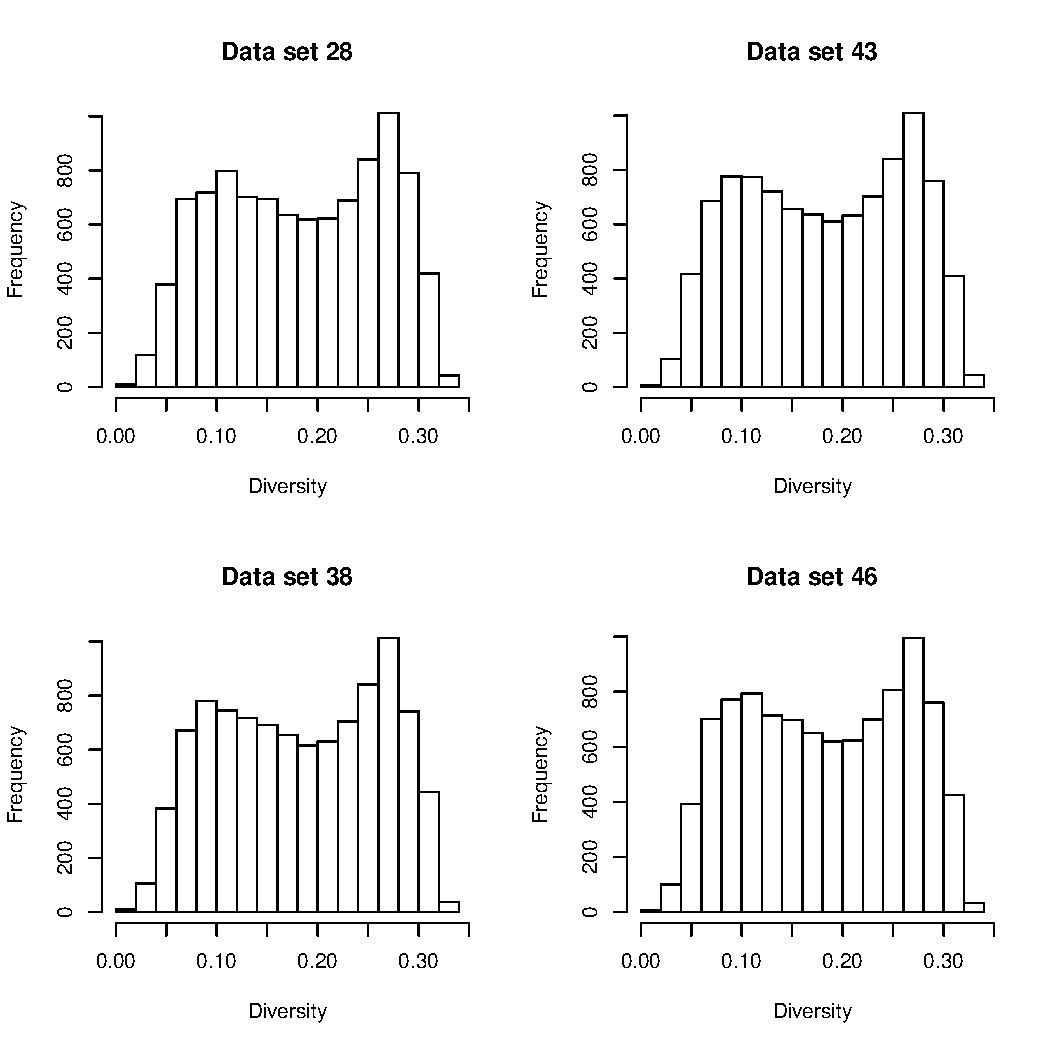
\includegraphics[width = .75\textwidth]{graphics/diver4hists.pdf}
\caption{histograms of the diversity measure in two (of 50) randomly selected data sets}
\end{figure}

\end{block}

\end{column} % End of column 2.1

\begin{column}{\onecolwid}\vspace{-.6in} % The second column within column 2 (column 2.2)

%----------------------------------------------------------------------------------------
%	INFERENCE
%----------------------------------------------------------------------------------------

\begin{block}{Prediction}

\begin{figure}[h]
 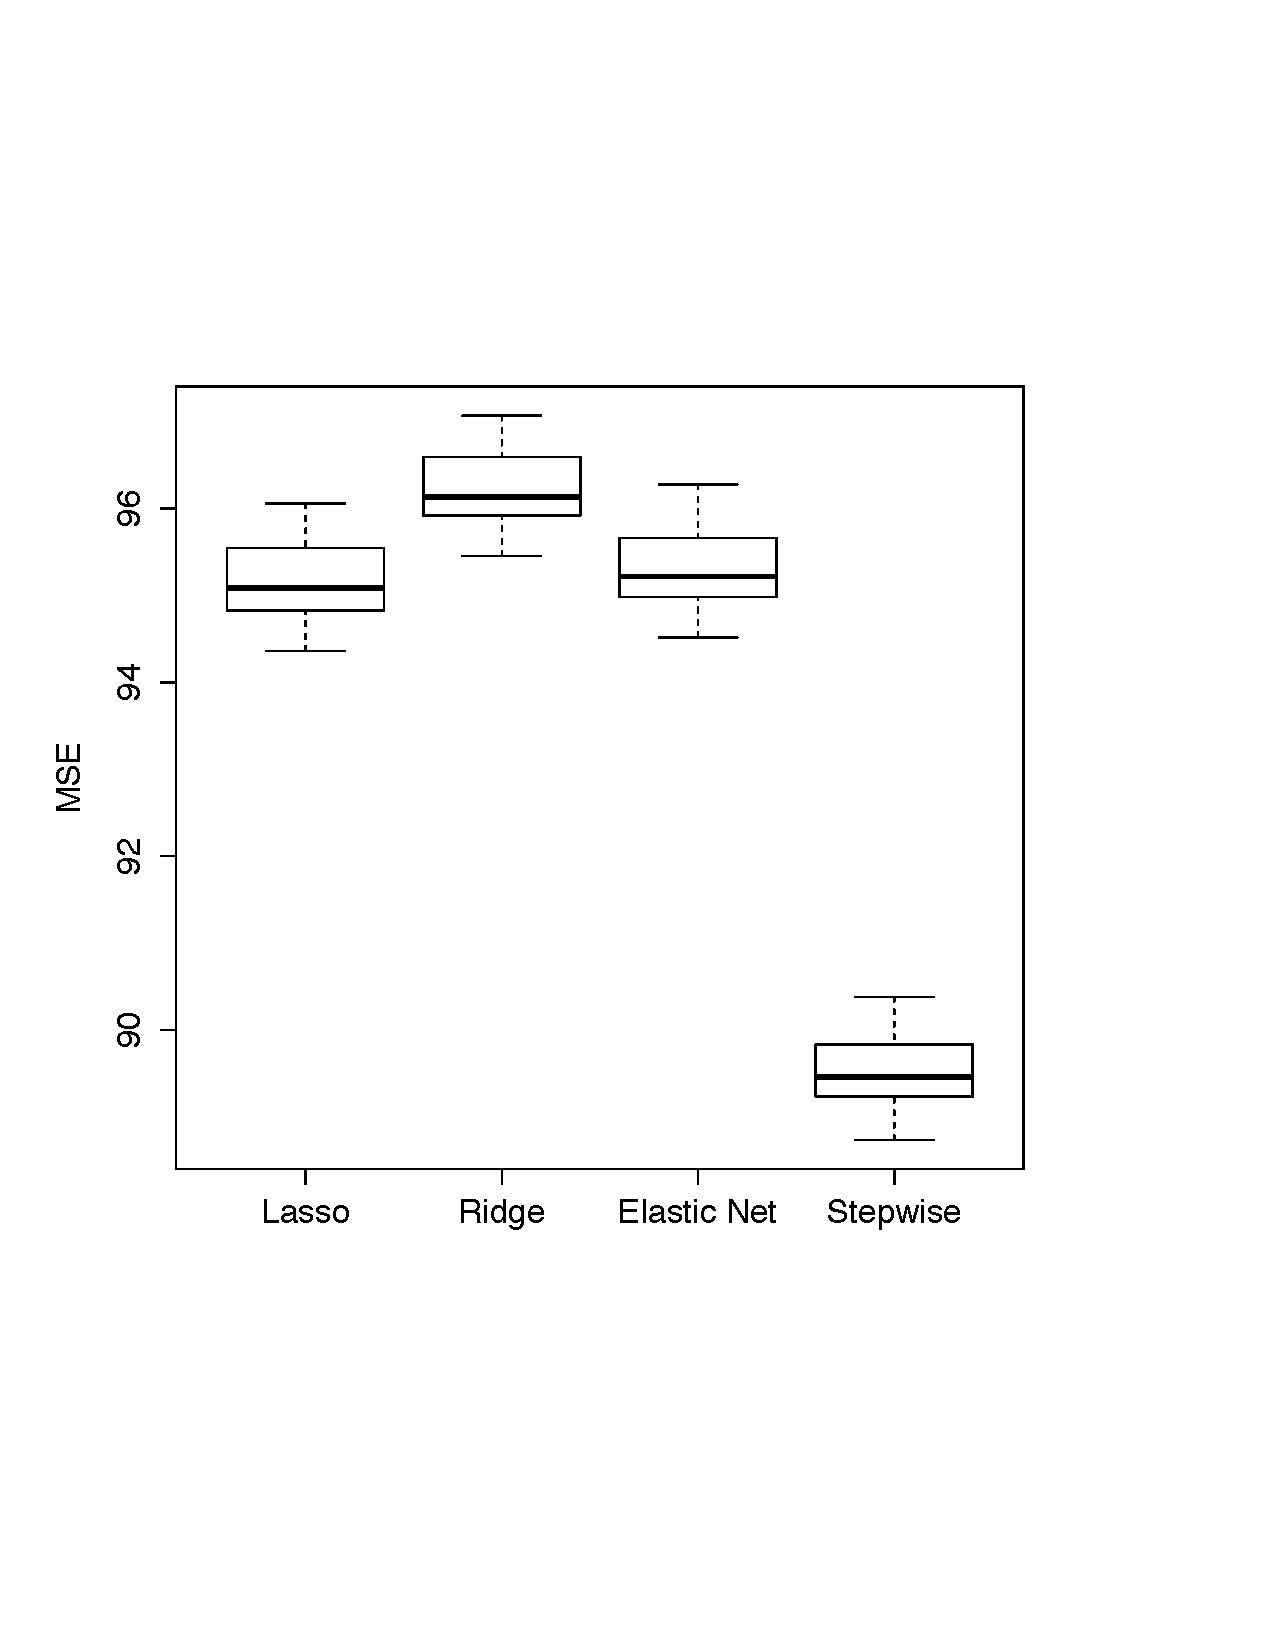
\includegraphics[width = .5\textwidth]{graphics/Prediction_BoxPlot.pdf}
\caption{Comparison of Mean Squared Errors \label{boxplot}}
\end{figure}

\begin{table}[ht]
\caption{Penalization values}
\label{lambda}
\centering
\begin{tabular}{r|rrrr}
  \hline
 & $\lambda_{min}$ & Var($\lambda_{min}$) & $\lambda_{1se}$ & Var($\lambda_{1se}$) \\ 
  \hline
Lasso & 0.04595 & 0.00006 & 0.27143 & 0.00505 \\ 
  Ridge & 1.46487 & 0.03459 & 6.77670 & 1.87964 \\ 
  Elastic Net & 0.08589 & 0.00025 & 0.54794 & 0.01765 \\ 
   \hline
\end{tabular}
\end{table}

\end{block}

%----------------------------------------------------------------------------------------

\end{column} % End of column 2.2

\end{columns} % End of the split of column 2 - any content after this will now take up 2 columns width


%----------------------------------------------------------------------------------------
%	IMPORTANT RESULT
%----------------------------------------------------------------------------------------

\begin{alertblock}{Important Result}

There is reasonable evidence that diversity at the district level as we have measured it seems to have a negative relationship with graduation rates.

\end{alertblock} 

%----------------------------------------------------------------------------------------

\begin{columns}[t,totalwidth=\twocolwid] % Split up the two columns wide column again

\begin{column}{\onecolwid} % The first column within column 2 (column 2.1)

%----------------------------------------------------------------------------------------
%	MATHEMATICAL SECTION
%----------------------------------------------------------------------------------------

\begin{block}{Mathematical Section}

We attempt to construct a general measure of diversity that will be high for racially diverse communities and low for racially homogeneous communities.  By doing this, we hope to construct results that can be seen without reference to specific ethnic groups.  We define the diversity statistic $D_j$ for community $j$ to be

\begin{equation}
 D_j = \prod_{i \in I}(1-x_{i,j}),
\label{eqn:Diversity Statistic}
\end{equation}

where $I$ is an indexing set for ethnic groups and $x_{i,j}$ is the proportion of ethnic group $i$ in community $j$.  We want to determine whether $D_j$ has a statistically significant impact on graduation rates once other factors are accounted for.  

\end{block}

%----------------------------------------------------------------------------------------

\end{column} % End of column 2.1

\begin{column}{\onecolwid} % The second column within column 2 (column 2.2)

%----------------------------------------------------------------------------------------
%	RESULTS
%----------------------------------------------------------------------------------------

\begin{block}{Inference}

The below table details the significance of our Diversity Statistic estimated coefficient for all our different regression models.

\begin{table}[ht]
\caption{Regression summary}
\label{regresults}
\centering
\begin{tabular}{rrrrrr}
  \hline
Model & Mean & Variance & Std. Error & t value & p value \\ 
  \hline
Linear 1 & -59.97 & 0.65 & 1.39 & -43.28 & 0.00 \\ 
  Linear 2 & -53.36 & 0.81 & 1.36 & -39.29 & 0.00 \\ 
  Linear 3 & -69.56 & 2.92 & 2.48 & -28.04 & 0.00 \\ 
   Linear 4 & -59.33 & 0.57 & 1.38 & -43.09 & 0.00 \\ 
  Linear 5 & -75.43 & 1.19 & 2.14 & -35.21 & 0.00 \\ 
  Linear 6 & -85.41 & 3.46 & 3.01 & -28.34 & 0.00 \\ 
  Lasso 1 & -45.04 & 2.18 & 1.47 & -30.57 & 0.00 \\
  Lasso 2 & -62.23 & 499.20 & 20.37 & -3.12 & 0.03 \\
  Lasso 3 & 62.38 & 530.68 & 22.11 & 2.87 & 0.06 \\
   \hline
\end{tabular}
\end{table}



\end{block}

%----------------------------------------------------------------------------------------

\end{column} % End of column 2.2

\end{columns} % End of the split of column 2

\end{column} % End of the second column

\begin{column}{\sepwid}\end{column} % Empty spacer column

\begin{column}{\onecolwid} % The third column

%----------------------------------------------------------------------------------------
%	CONCLUSION
%----------------------------------------------------------------------------------------

\begin{block}{Conclusion}

We can see that our diversity statistic does indeed have a negative impact on graduation rates at the county level. Given that our data is public domain, we suspect that the bidirectional-elimination or lasso model would accurately predict graduation rates in future years. Furthermore, our model could be improved with a time series analysis of graduation rates along with our covariates over a number of years.

\end{block}

%----------------------------------------------------------------------------------------
%	LIMITATIONS & NEXT STEPS
%----------------------------------------------------------------------------------------

\begin{block}{Limitations}

There are various potential issues with our methods and resulting conclusion, including:
\begin{itemize}
\item Ecological Inference Problem
\item Omitted Variable Bias
\item Data Imputation Methods
\end{itemize}



\end{block}




%----------------------------------------------------------------------------------------
%	ACKNOWLEDGEMENTS
%----------------------------------------------------------------------------------------

\setbeamercolor{block title}{fg=red,bg=white} % Change the block title color

\begin{block}{Acknowledgements}

\small{\rmfamily{I would first like to thank AT\&T and the Data for Diplomas project for providing such a rich and interesting dataset to work on. I would like to acknowledge Professor Sayan Mukherjee for challenging me with my methods and results. I would also like to thank Sunith Suresh, Azeem Zaman, and Lin Xiao, with whom I worked on part of this project with in our Predictive Modeling course.}} \\

\end{block}

%----------------------------------------------------------------------------------------
%	CONTACT INFORMATION
%----------------------------------------------------------------------------------------

\setbeamercolor{block alerted title}{fg=black,bg=norange} % Change the alert block title colors
\setbeamercolor{block alerted body}{fg=black,bg=white} % Change the alert block body colors

\begin{alertblock}{Contact Information}

\begin{itemize}
\item Email: \href{mailto:sanjay.hariharan@duke.edu}{sanjay.hariharan@duke.edu}
\item Phone: +1 (414) 828 3096
\end{itemize}

\end{alertblock}

\begin{center}
\begin{tabular}{ccc}

\includegraphics[width=0.8\linewidth]{graphics/duke_logo.png}
\end{tabular}
\end{center}

%----------------------------------------------------------------------------------------

\end{column} % End of the third column

\end{columns} % End of all the columns in the poster

\end{frame} % End of the enclosing frame

\end{document}
